\section{Theorie}
\label{sec:Theorie}
\subsection{Ziel}
\label{subsec:Ziel}
In diesem Versuch wird der Diodenlaser eingestellt, dass dieser mit einer Energie abstrahlt, bei welcher Fluoreszenz bei Rubidium beobachtet werden kann. 
Außerdem wird das Absorptionsspektrum von Rubidium aufgenommen.
\subsection{Prinzipielle Funktionsweise eines Diodenlasers}
\label{subsec:prinzipielleFunktionsweise}
Grundlegend für einen Laser ist die Populationsinversion. Eine Populationsinversion liegt z.B. bei einem 2 Niveausystem vor, wenn in diesem System mehr Teilchen
in dem Niveau 2 mit der Energie $E_2$ als in dem Niveau 1 mit der Energie $E_1$, wobei $E_2 > E_1$ gilt, sind.
Wenn ein Teilchen von Niveau 2 auf Niveau 1 springt, wird aufgrund der Energieerhaltung ein Photon mit der Energie $E_2 - E_1 = \hbar\omega$ abgestrahlt.
Die Abstrahlung eines Photons wird Emission genannt, wobei bei dem Laser die stimulierte Emission genutzt wird, da diese koheräntes Licht abstrahlt, welches bei einem Laser
von großer Bedeutung ist. 
Die stimulierte Emission wird durch ein Photon verursacht, weswegen ein Photon erzeugt wird, welches die gleiche Wellenlänge,
Phase, Polarisation und Ausbreitungsrichtung besitzt. 
Somit ist das emittierte Licht koheränt.
\subsection{Komponenten eines Diodenlasers}
\label{subsec:Komponenten}
\begin{figure}
    \centering
    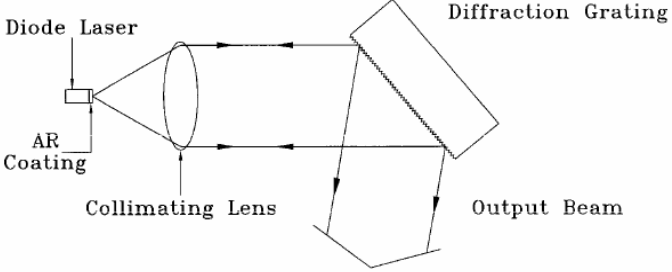
\includegraphics[width = 0.78\textwidth]{pictures/komponenten.png}
    \caption{Grober Aufbau eines Diodenlasers\cite{theorie}}
    \label{pic:theorie}
\end{figure}
Ein Diodenlaser (Laser ist ein Akronym für light amplification by stimulated emission of radiation) besteht im wesentlichen aus 3 Komponenten. 
Diese sind das aktive Medium\ref{subsubsec:aktivesMedium}, der interne Resonator\ref{subsubsec:internerResonator} 
und der externe Resonator bzw. das Gitter\ref{subsubsec:externeResonator}.
\subsubsection{Aktive Medium}
\label{subsubsec:aktivesMedium}
In dem aktiven Medium werden Photonen durch p-n-Übergänge erzeugt. P-dotierte Halbleiter sind mit einem Element, welches ein Valenzelektron weniger besitzt, versehen. 
Dieses fehlende Elektron kann als Loch (positiv geladenes Quasiteilchen) behandelt werden.
Das Loch wird durch ein Valenzelektron eines Halbleiteratoms aufgefüllt, wodurch sich dieses schon bei geringen Temperaturen fortbewegen kann, da an diesem Halbleiteratom ein Loch enstanden ist,
welches wieder aufgefüllt wird. Deshalb wird das Fremdatom auch Akzeptor genannt.
Bei der n-Dotierung wurde dem Halbleiter ein Element hinzugefügt, welches ein Valenzelektron mehr besitzt. Dieses kann sich ebenfalls schon bei geringen Temperaturen frei bewegen,
weshalb dieses Fremdatom Donator genannt wird.
Entscheident bei dem Laser ist der p-n-Übergang, welcher durch Kontakt einer p-dotierten und einer n-dotierten Halbleiterschicht entsteht.
\begin{figure}
    \centering
    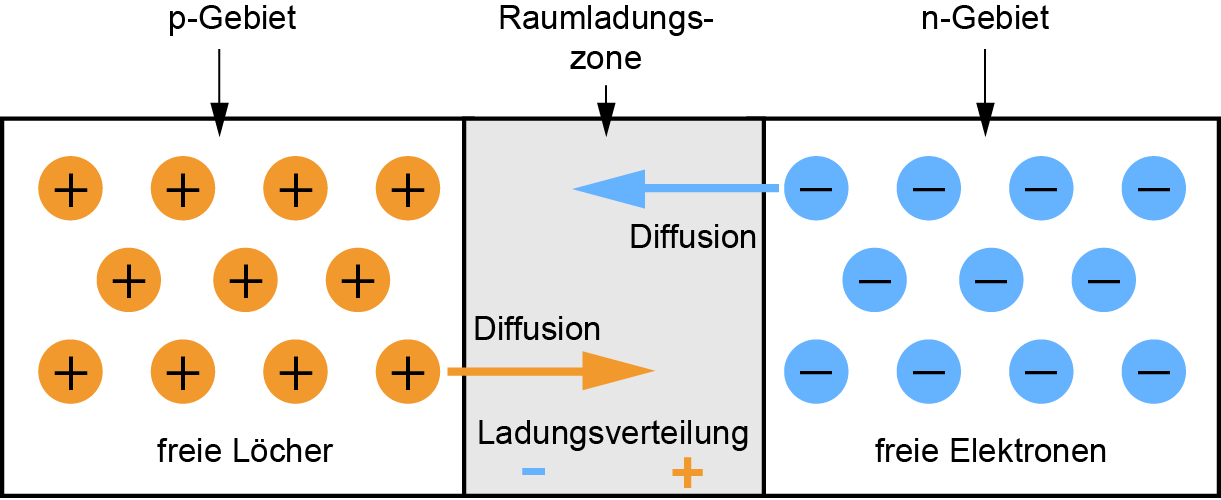
\includegraphics{pictures/p-n-uebergang}
    \caption{Diffusion bei Kontakt zwischen einem n- und p-dotierten Halbleiter\cite{p-n-uebergang}}
    \label{pic:diffusion}
\end{figure}
Dabei diffundieren die überschüssigen Elektronen der n-dotierten in die p-dotierte Schicht, während die überschüssigen Löcher des p-dotierten Halbleiters in die n-dotierte
Schicht diffundieren.
Dadurch fehlen in den jeweiligen Schichten frei bewegliche Ladungsträger und die ortsfesten Dotierungsatome sind nicht mehr elektrisch neutral.  
Somit entsteht eine Raumladungszone mit einer inhomogenen Ladungsverteilung, wodurch eine Spannung erzeugt wird.
Diese Spannung dient für die freien Ladungen als Potentialwall. Das Elektron in Abbildung \ref{pic:kruemmung} kann die Raumladungszone nur überqueren, wenn es die Energie $E_C$ besitzt
, wonach es mit einem Loch rekombinieren kann und Energie, die mindestens der Bandlücke entspricht, in Form von einem Photon abstrahlt.
\begin{figure}
    \centering
    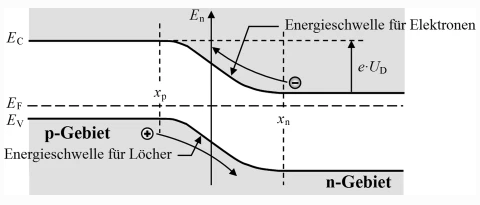
\includegraphics[width = 0.78\textwidth]{pictures/kruemmung.png}
    \caption{Die Krümmung der Baender bei Kontakt von p- und n-dotierten Halbleitern\cite{kruemmung}}
    \label{pic:kruemmung}
\end{figure}
Wird nun eine externe Spannung angelegt, wobei der negative Pol an die n-dotierte und der positive Pol an die p-dotierte Schicht angelegt wird, wird diese Spannung vermindert,
wodurch die freien Ladungen weniger Energie benötigen, um die Raumladungszone zu überqueren.
Bei umgedrehter Polung würde die Potentialdifferenz erhöht, wodurch die freien Ladungen noch mehr Energie benötigen würden.
\subsubsection{Interner Resonator}
\label{subsubsec:internerResonator}
Der interne Resonator wird durch die gegenüberliegenden Ränder des Kristalls in horizontaler Richtung gebildet, welche eine verschiedene Reflektivität besitzen.
Dadurch kann am richtigen Rand Licht austreten, während an dem anderen Ende kein Licht transmittiert wird.
Dadurch kann eine reflektierte Welle durch stimulierte Emission weitere Photonen auslösen.
Damit der interne Resonator tatsächlich als Verstärker dient,
muss sich dort eine stehende Welle ausbreiten, für welche die Randbedingung 
\begin{equation}
    \psi \left (kL \right ) \overset{!}{=} 0    \label{eqn:psi}
\end{equation}
gilt. In dieser eindimensionalen Betrachtung ist $\psi$ die Amplitude, $k$ die Wellenzahl und $L$ die Länge des Resonators bzw. Kristalls ist. 
Daraus folgt, dass die Wellen eine Wellenlänge von 
\begin{equation}
    \lambda = 2\frac{L}{n}, \; \; \; n \in \symbb{N} \label{eqn:lambda}
\end{equation}
haben müssen.
\subsubsection{Externer Resonator/Gitter}
\label{subsubsec:externeResonator}
Die kollimierende Linse sorgt dafür, dass die Strahlen annähernd kolinear verlaufen, so dass der Laserstrahl gebündelt ist.
An dem Gitter sind die duch Interferenz enstehenden Beugungsmaxima 0. und 1. Ordnung von Relevanz.
Das 0. Maximum wird reflektiert, so dass dieses Licht zum Experimentieren genutzt werden kann. Das 1. Maximum wird bei der richtigen Wellenlänge zurück zum Kristall reflektiert.
Hierbei gilt die Bragg-Bedingung
\begin{equation}
   k \cdot \lambda = 2d \sin \left (  \theta \right ) , \; \; \; k \in \symbb{N} \label{eqn:bragg} ,
\end{equation}
wobei $d$ die Gitterkonstante, $k$ die Ordnung des Maximus und $\theta$ der Beugungswinkel ist.
Dieser externe Resonator wird durch die weniger reflektierende Seite des Kristalls und dem Gitter gebildet.
Die Funktionsweise ist hierbei dieselbe und die Relationen \ref{eqn:psi} und \ref{eqn:lambda} gelten auch hier, wobei $L$ jetzt nicht mehr die Länge des Kristalls, sondern 
der Abstand des Gitters zum Kristall ist.
\subsection{Leistung}
\begin{figure}
    \centering
    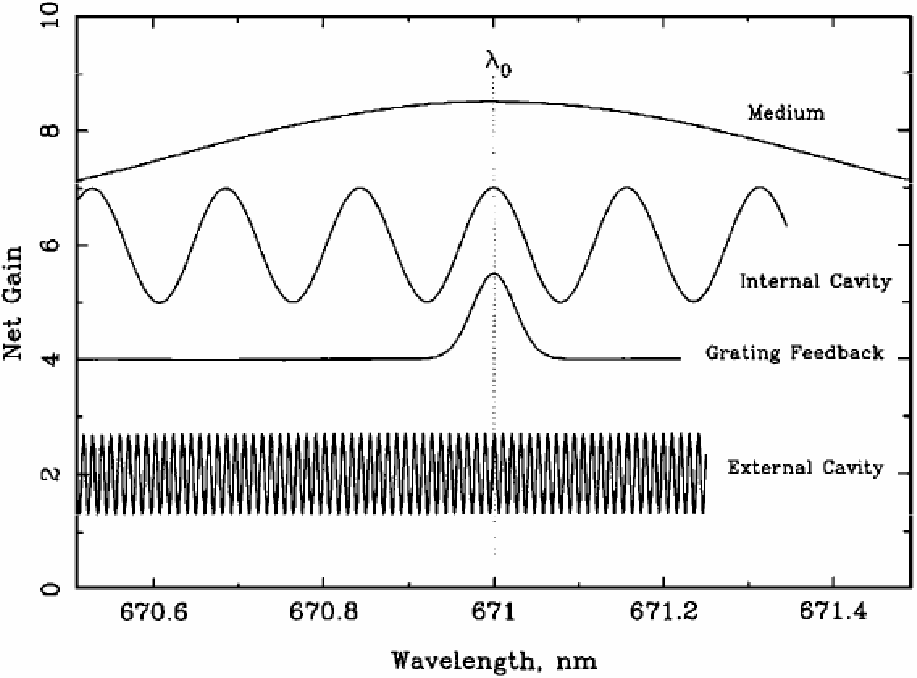
\includegraphics[width = 0.78\textwidth]{pictures/gain.png}
    \caption{Die jeweiligen Leistungen der einzelnen Komponenten in Abhängigkeit von der Wellenlänge\cite{theorie}}
    \label{pic:gain}
\end{figure}
Das in der Abbildung \ref{pic:gain} zu sehende Maximum der Kurve des Mediums, lässt sich auf die Bandlücke zurückführen. 
Diese Photonen haben die zu der Wellenlänge $\lambda_0$ gehörende Energie, welche der Bandlücke entspricht. 
Da die Bandstruktur jedoch kontinuierlicher und nicht diskreter Natur ist, ist das Maximum ein sehr breites Maximum.
Die Periodizität des internen und externen Resonators lässt sich mit der Bedingung \ref{eqn:lambda} erklären, da nur Wellen mit einer am Rand verschwindenden Amplitude zur Leistung stark beitragen.
Die höhere Frequenz der Kurve von dem externen Resonator in Abbildung \ref{pic:gain} lässt sich ebenfalls mittels \ref{eqn:lambda} erklären, da die 
 
\subsection{Einflüsse auf die Wellenlänge}
\subsubsection{Temperatur}